%%%%%%%%%%%%%%%%%%%%%%%%%%%%%%%%%%%%%%%%%%%%%%%%%%%%%%%%%%%%%%%%%%%%%%%
%%%%%%%%%%%%%%%%%%%%%%%%%%%%%%%%%%%%%%%%%%%%%%%%%%%%%%%%%%%%%%%%%%%%%%%
%%%%%                                                                 %
%%%%%     <file_name>.tex                                             %
%%%%%                                                                 %
%%%%% Author:      <author>                                           %
%%%%% Created:     <date>                                             %
%%%%% Description: <description>                                      %
%%%%%                                                                 %
%%%%%%%%%%%%%%%%%%%%%%%%%%%%%%%%%%%%%%%%%%%%%%%%%%%%%%%%%%%%%%%%%%%%%%%
%%%%%%%%%%%%%%%%%%%%%%%%%%%%%%%%%%%%%%%%%%%%%%%%%%%%%%%%%%%%%%%%%%%%%%%

\chapter{Introduction}

The Hyperloop Passenger Transportation Concept was initially proposed by Elon Musk in his Hyperloop Alpha paper\cite{HyperloopAlpha} as an alternative to the planned high-speed rail project connecting San Francisco and Los Angeles. It was argued that the high-speed rail project is not state of the art in terms of technology, it is much too expensive and significantly slower than other high-speed trains around the world. The objective of the Hyperloop is to achieve passenger transport on the ground over long distances at speeds exceeding 1220 km/h.

To achieve such high speeds, pressurized passenger capsules ("pods") would run in tubes where near vacuum is maintained. The initial proposal also called for air-bearings to allow the pod to levitate during transit. In order to supply the air bearings with pressurised air and further reduce drag, a compressor would suck the remaining air in through an inlet at the front of the pod. A linear motor system would be used to accelerate and decelerate the pod at high speeds while limiting the acceleration to 1g for passenger comfort.

\section{Hyperloop Competition}

Although the Hyperloop Alpha proposal was turned down, SpaceX decided in 2015 to hold a student competition\cite{HyperloopCompetiton} in order to drive the development of Hyperloop technology. To this end they constructed a 1,25km test tube designed to reach an ambient pressure of 8mBar. The tube features an aluminium sub-track and rail mounted on a concrete fill bed.

\begin{figure}[H]
  \centering 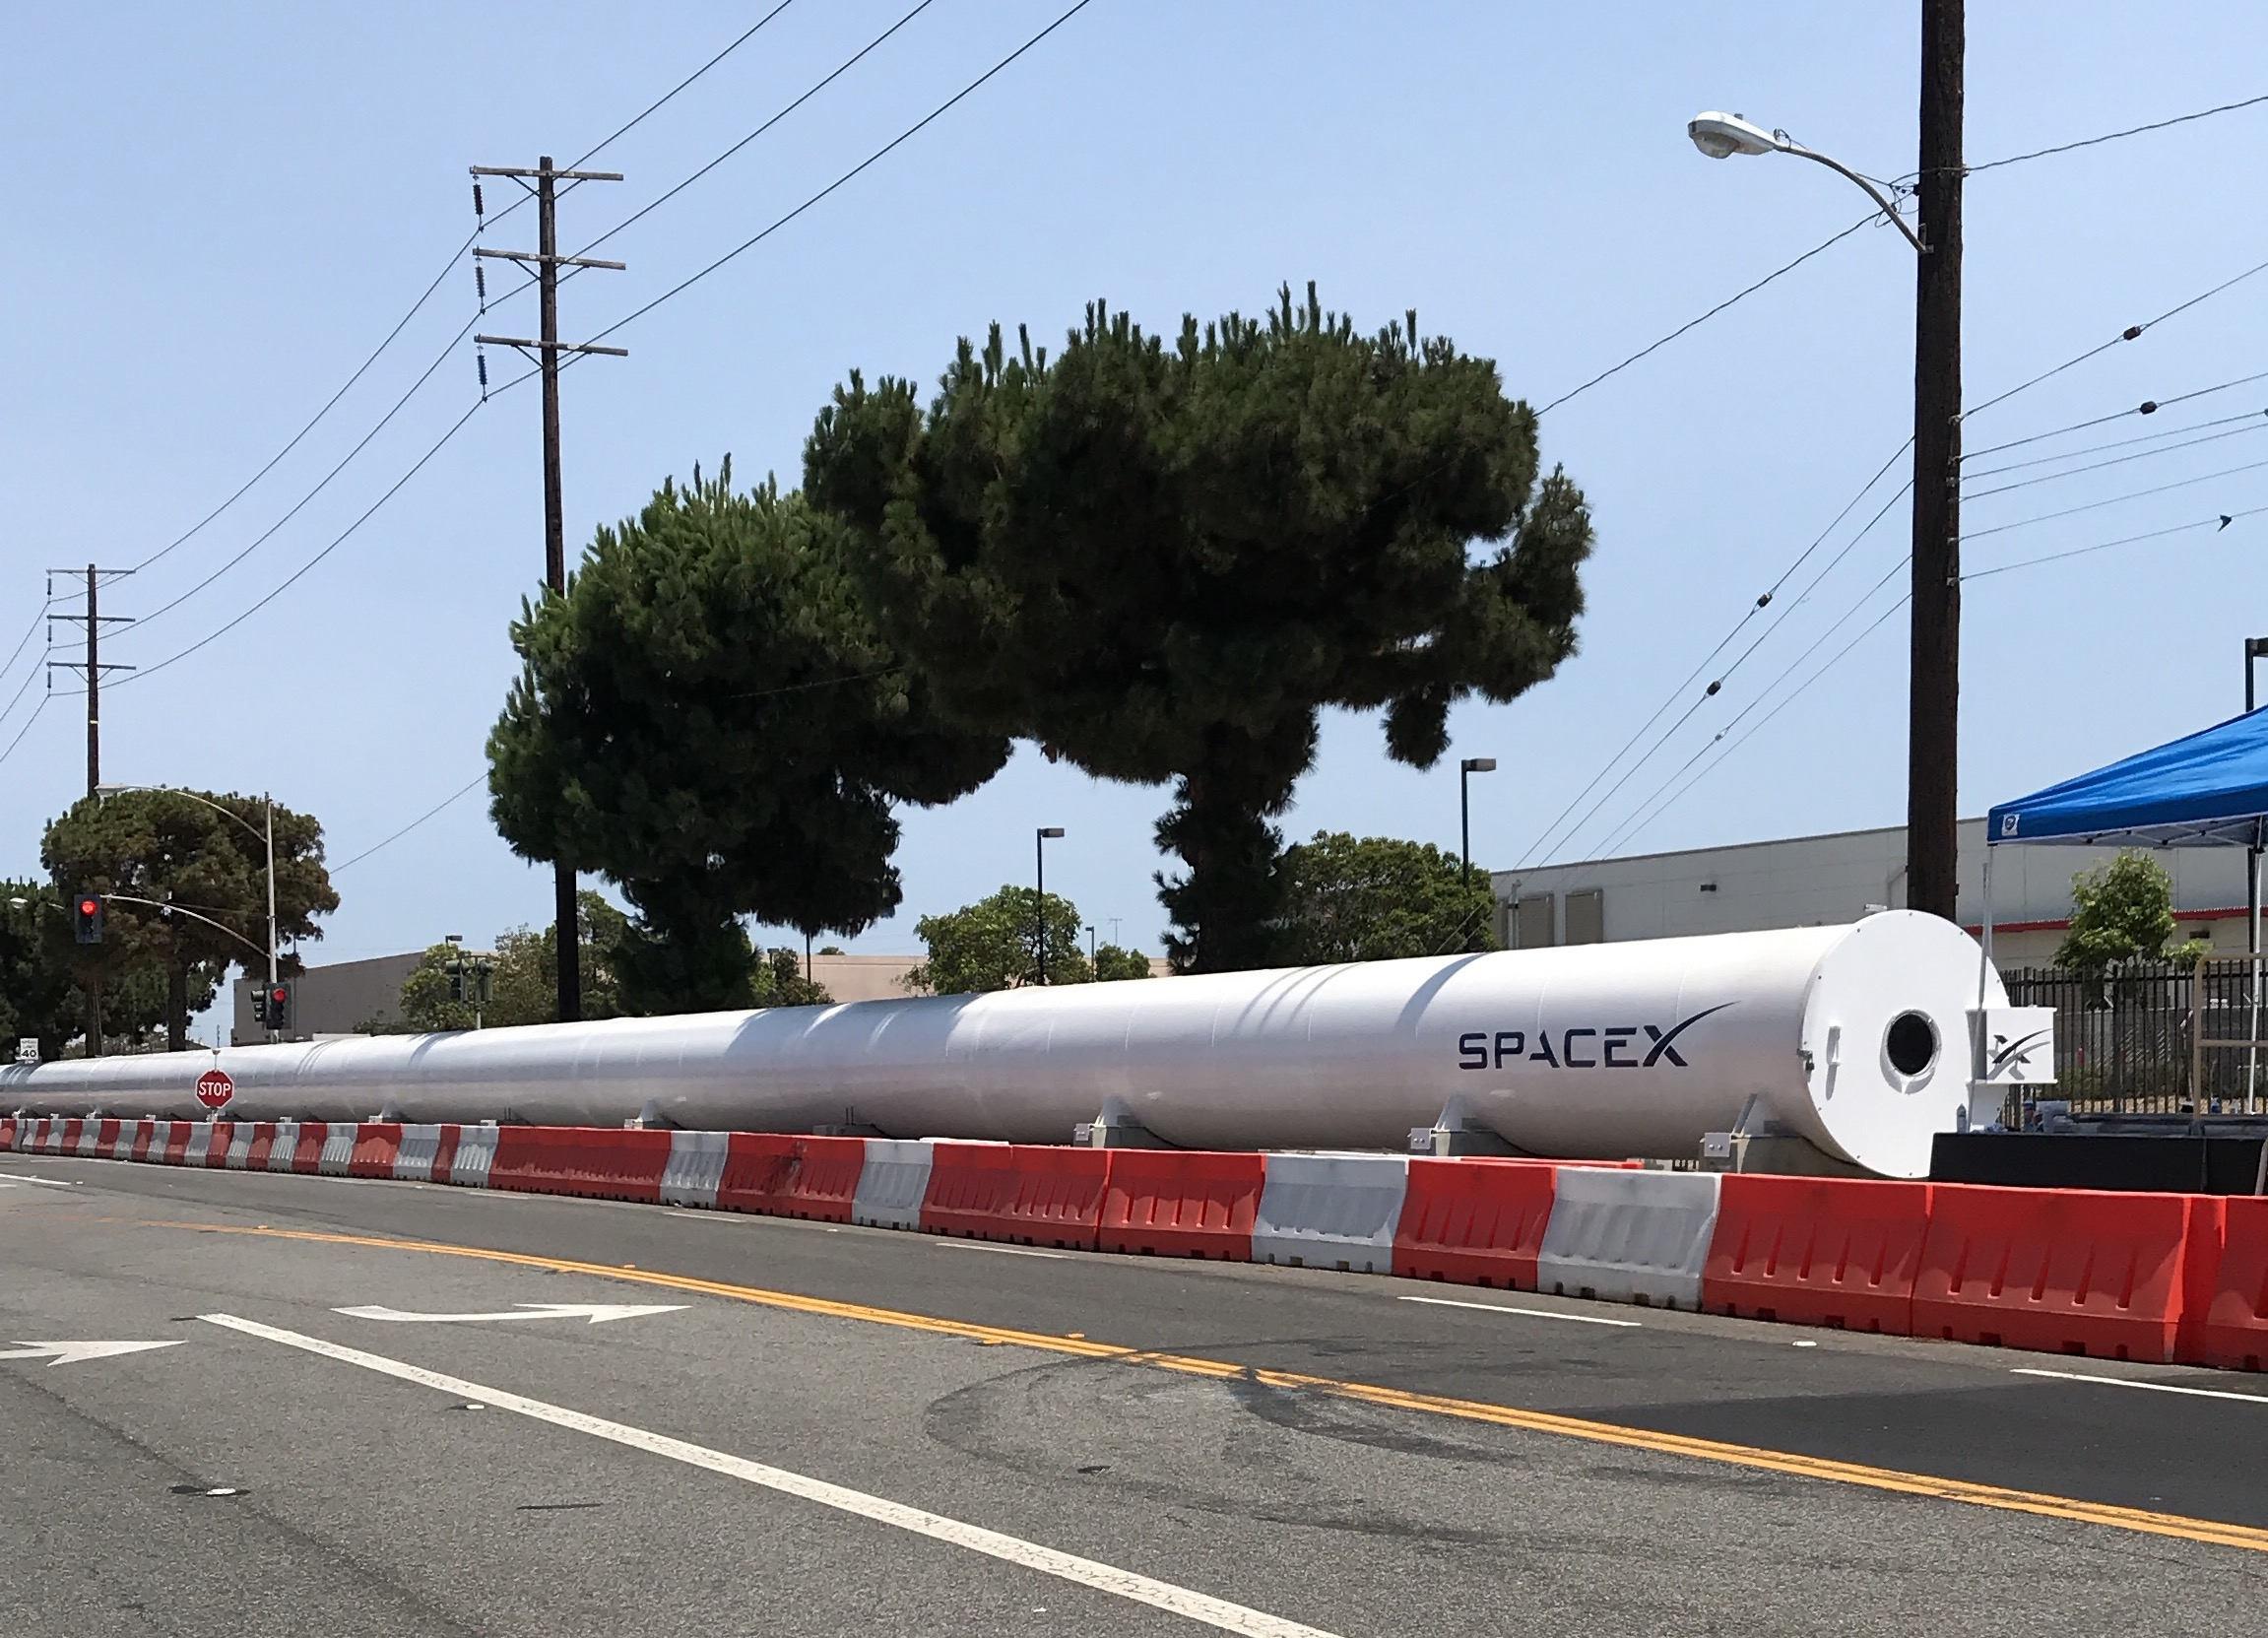
\includegraphics[width=1.0\textwidth]{./figures/hyperloop_tube}
  \caption{Hyperloop test tube at SpaceX headquarters in Los Angeles.}
\end{figure}

Since the first competition there have been a second and third iteration and a forth has been announced for the summer of 2019.

The objective for the teams is to build a prototype Hyperloop pod and race it in the test tube. The pod reaching the highest velocity with successful deceleration wins the competition. During the first and second competition, a pusher vehicle was available to accelerate the pods to a pre-defined velocity at the beginning of their run. Therefore, it was optional for a pod to incorporate a propulsion system. However, in the third competition the pods were required to accelerate independently.

The first step of the competition is the Preliminary Design Briefing in which the team must outline the main concepts of their pod design. After it has been approved teams may proceed to submit the Final Design Briefing a few months later. This must include all details of the pod's design and show that the design is safe. Approximately 20 teams are then selected to compete in the competition at SpaceX headquarters in Los Angeles.

The competition in Los Angeles consists mostly of a testing week where the pod must pass a series of tests to prove safety and correct operation before being allowed to enter the test tube. The most promising teams are then selected to compete in the final on the last day of the competition. Here teams aim to reach the highest speed in order to win the competition.

\section{Swissloop}

Swissloop\cite{Swissloop} was founded as an association in September 2016 by a group of ETH Zurich students with the intention of competing in the second iteration of the Hyperloop Pod Competition. Swissloop was able to gain support from many industry sponsors and several departments at ETH Zurich including the Integrated Systems Laboratory. In July 2017 Swissloop revealed it's first pod Escher to the public. After reaching the finals of the competition with Escher in August 2017, a new team was assembled to compete in the third competition in July 2018 with a completely new pod called Mujinga.

\subsection{Escher}

Swissloop's first pod featured a cold gas propulsion system which was designed for a second acceleration stage after the initial acceleration delivered by the pusher. The pod also featured hydraulic bakes as well as a passive levitation system.

The avionics implemented for Escher included around 30 sensors and provided a reliable basis for controlling the pod. Although eventually several flaws became apparent, the system provided a solid basis for the development of the avionics system of Mujinga. While Mujinga retained some components of the hardware, the design ended up being completely different in several ways. The Software was almost entirely rewritten from the ground up leading to large performance and reliability improvements.

\begin{figure}[H]
  \centering 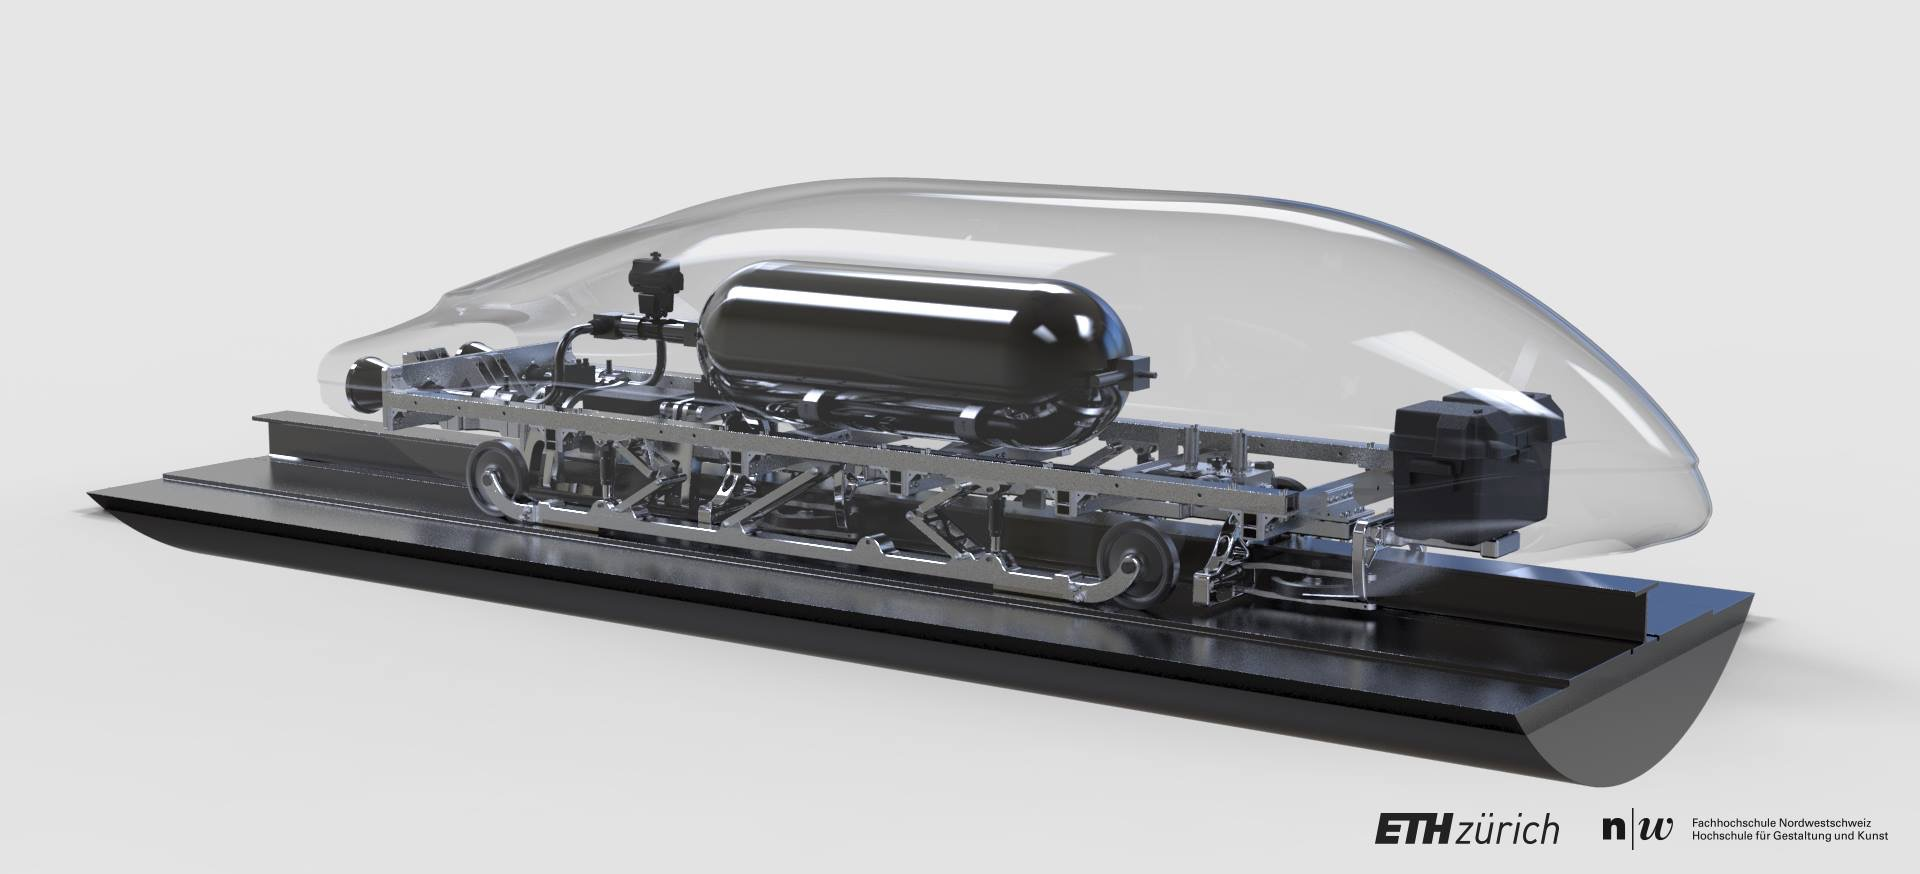
\includegraphics[width=1.0\textwidth]{./figures/escher_transparent}
  \caption{Rendering of Escher with transparent shell.}
\end{figure}

\subsection{Mujinga}

Swissloop's second pod design builds on the lessons learned with Escher but includes many significant changes. Most noticeable, Mujinga no longer levitates but uses wheels and four electric motors as a propulsion system. Two high-voltage (700V) batteries produce 500kW of power to accelerate to a top-speed of 500km/h. Similar but redesigned hydraulic brakes decelerate the pod before the end of the 1,25km test track. A pneumatic clamping system presses the pod against the track to produce the down-force necessary to achieve the necessary acceleration.

As mentioned, the avionics system was based on the platform used in Escher. However, much emphasis was placed on greater simplicity and reducing bottlenecks. A problem with the logging system in Escher meant that the amount of data that could be acquired was very small. Therefore, the logging system in Mujinga was specifically designed to handle much higher data rates.

\begin{figure}[H]
  \centering 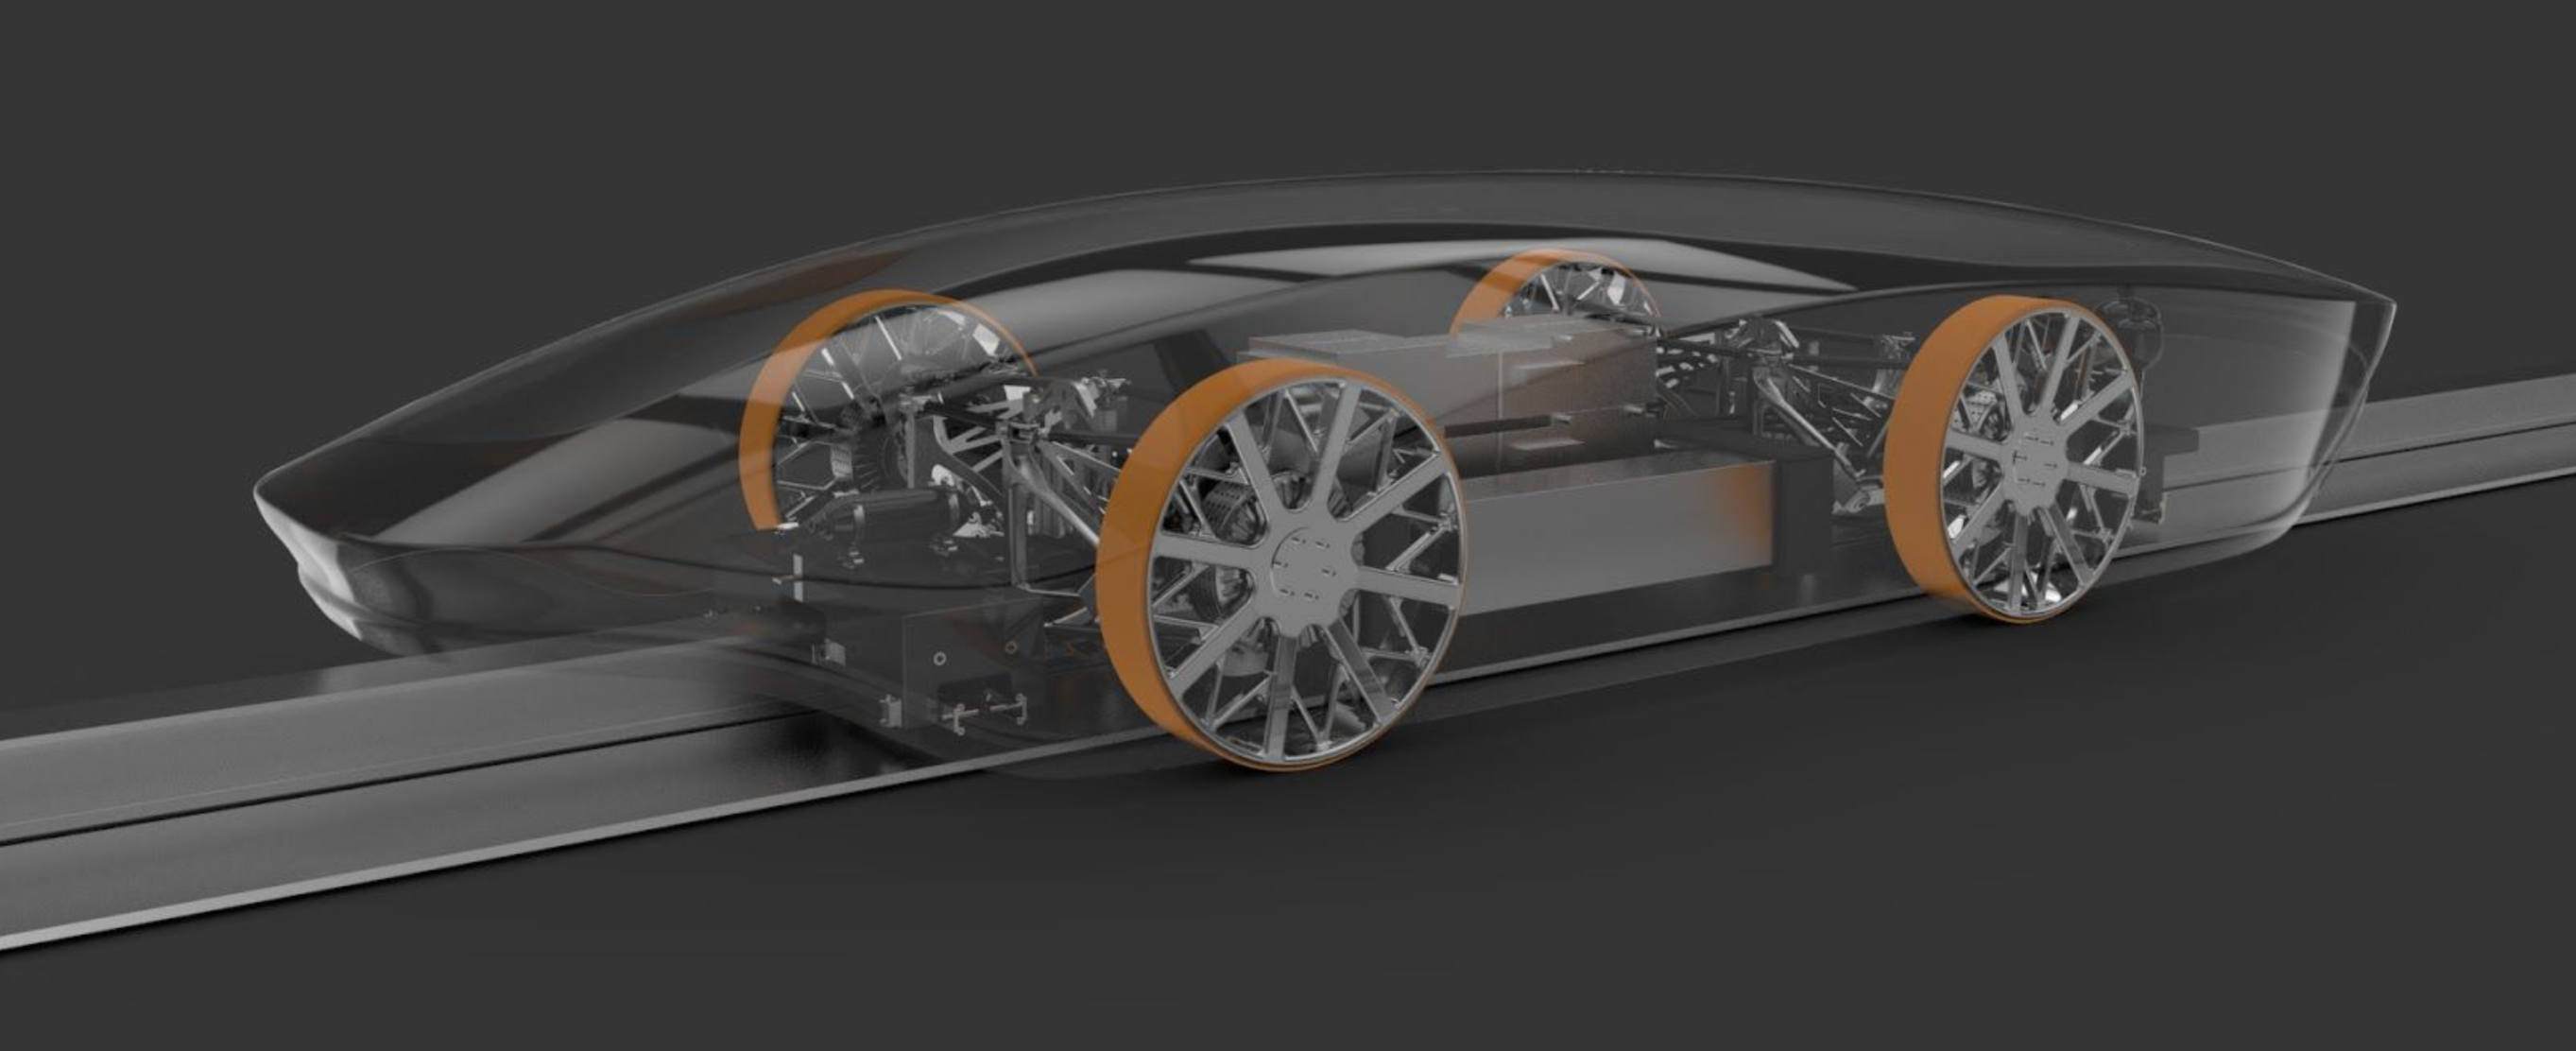
\includegraphics[width=1.0\textwidth]{./figures/mujinga_transparent}
  \caption{Rendering of Mujinga with transparent shell.}
\end{figure}

\begin{figure}[H]
  \centering 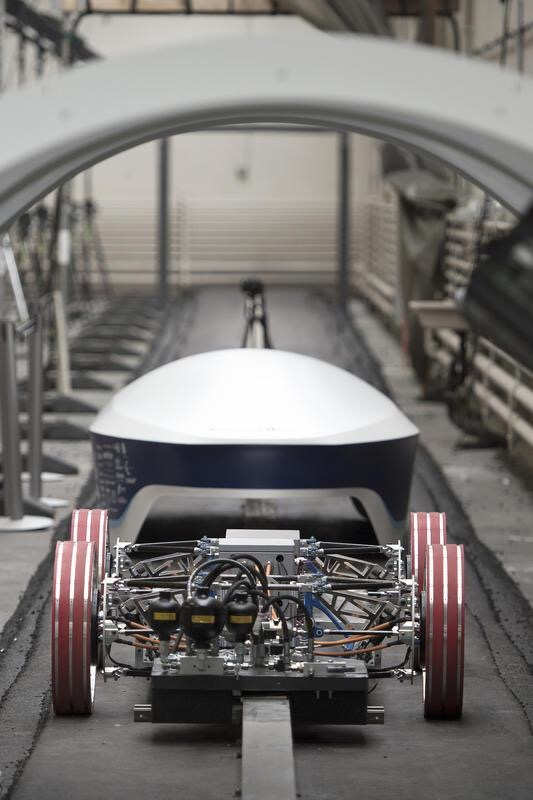
\includegraphics[width=0.5\textwidth]{./figures/mujinga_noshell}
  \caption{Picture of Mujinga with separated shell.}
\end{figure}

\section{Project Scope}

The scope of this Bachelor Thesis is the implementation of the avionics and control software running on the Hyperloop pod. This includes the following tasks:

\begin{itemize}
    \item Platform selection
    \item Development of drivers to interface and communicate with on-board sensors
    \item Development of drivers for a network interface and SD card
    \item Development of drivers for communication with motor controllers (inverters), battery management systems and brake actuators
    \item Implementation of a control scheme which ensures safe and correct operation of the pod while executing traction control and yaw control algorithms (developed by team members)
    \item Implementing communication with a control panel (developed by another team member) over a network and logging all collected data, as well as system events
\end{itemize}

The following tasks are not part of this bachelor thesis and were completed by other people:

\begin{itemize}
    \item Design of custom PCBs (Hanno Kappen)
    \item Development of traction control (Julius Wanner and Stefan Weber) and yaw control algorithms (Yannick Strümpler)
    \item Development of a control panel for visualizing telemetry and controlling the pod (Laurin Paech)
    \item Wireless network for communication with the pod (SpaceX)
\end{itemize}

The control system in this thesis was developed specifically for the Hyperloop Pod Student Competition. As such it was tested in the field as part of the Mujinga pod at testing facilities in Switzerland and at the competition in Los Angeles at SpaceX's headquarters.

%%% Local Variables: 
%%% mode: latex
%%% TeX-master: "../report_template"
%%% End: 
